% O TEXTO ABAIXO É REFERENTE À SEÇÃO 2.5 (BACHOR - EXPERIMENTS IN QUANTUM OPTICS - PHOTODECTECTION TECHNIQUES). ESTÁ EM "LIXO RECICLÁVEL" PORQUE FICOU MAL ESCRITO.


\begin{displayquote}
    Em laboratório, a luz não é detectada diretamente: é quase sempre convertida em sinais elétricos, que por sua vez são detectados e analisados.
\end{displayquote}

Há duas classes de métodos para detecção de luz: \textbf{detecção de campo}, que envolve medições de amplitude e fase, e \textbf{detecção de intensidade}, em que nenhuma informação de fase é coletada.

Para energias menores do que na faixa de \textit{mid-IR}, a detecção de campo pode ser feita diretamente. Para energias maiores, a detecção é feita indiretamente por técnias de \textbf{detecção homodina ou heterodina}, em que o campo em questão interfere com um campo de referência com ampitude e fase conhecidas, e o campo resultante é analisado com detectores de intensidade.

\subsection{Características de Fotodetectores}

\textit{Grosso modo}, há duas formas de registrar a intensidade da luz: detectando fótons individuais ou medindo correntes. De qualquer forma, há algumas características essenciais de qualquer fotodector.

\subsubsection{Eficiência Quântica}

É a probabilidade de que a luz incidente seja convertida a um sinal mensurável:

\begin{equation}
    \text{taxa dos pulsos de Sinal}=\eta_{det}\text{taxa de fótons incidentes}
\end{equation}

É um parâmetro fundamental em muitos experimentos de óptica quântica. Evidentemente, se $\eta<1$, então uma corrente perfeitamente regular será medida como uma série de pulsos razoavelmente randomizado.

A eficiência quântica depende do material, da geometria do detector e do comprimento de onda da luz incidência.

\subsubsection{Dark Noise}

Mesmo na ausência de luz, fotodetectores ainda produzem algum sinal. Entre as possíveis causas: efeitos térmicos, impurezas nos materiais e campos "perdidos". Para experimentos de fotodetecção à temperatura ambiente, a temperatura é frequentemente reduzida para limitar o ruído.

\subsubsection{Rapidez e Saturação}

É útil definir alguns tempos de resposta dos fotodetectores:

\begin{equation*}
    \text{tempo de excitação}\rightarrow \tau_\varepsilon
\end{equation*}

Que é o tempo que um detector leva para excitar um sinal mensurável.

\begin{equation}
    \text{dead time}\rightarrow \tau_{\Delta}
\end{equation}

Que é o tempo que um detector leva para se recuperar antes de poder ser excitado novamente. Uma taxa de contagem muito alta, em comparação com o \textit{dead time}, deve levar à saturação.

\subsection{Detectando Fótons Individuais}

Fótons individuais carregam quantidades muito pequenas de energia ($10^{-19} J$ para um fótons de luz visível com $\nu=10^{15} Hz$). Para detectá-los, algumas técnicas são necessárias. Nessa seção, discutimos técnicas (1) \textbf{fotoquímicas}, (2) \textbf{fotoelétricas}, (3) \textbf{fototérmicas} e (4) \textbf{fotoópticas}.

\subsubsection{Detectores Fotoquímicos}

A energia de um único fóton é suficiente para induzir uma alteração química em uma porção de filme fotográfico. A técnica tem alta resolução, baixo ruído e boa resolução espacial, entretanto não permite monitoramento em tempo real do experimento.

\subsubsection{Detectores Fotoelétricos}

O dispositivo mais comum para transformar fótons em correntes elétricas mensuráveis é o PMT (\textit{photo multiplier tube}),  já bem conhecido. São dispositivos com boa rapidez, baixo \textbf{dark noise} e largura de banda alta. A eficiência, entretanto, é muito baixa.

Uma versão do PMT com eficiência mais alta é o \textit{Avalanche Photo Diode} (APD), que é o análogo semicondutor do PMT, construído utilizando um material com uma largura de banda menor que a energia dos fótons medidos.

\subsubsection{Detectores Fototérmicos}

Dispositivos que absorvem luz e a convertem em calor. Funcionam a partir de materiais supercondutores, operando em temperaturas próximas à de transição. A absorção de um único fóton é suficiente para levar o material de volta ao regime normal de condução, e a forte mudança em impedância pode ser medida.

\subsection{Detectando Fotocorrentes}

Começamos com a definição da fotocorrente, que dá a taxa em que os fótons chegam até o detector:

\begin{equation*}
    i(t)=\frac{n_e(t) e}{\Delta t}=\frac{P(t)e}{h\mu\eta_{det}}
\end{equation*}

Onde $\eta$ é a eficiência de conversão do detector. Naturalmente, estamos interessados na média $\bar{i}=\langle i(t) \rangle$, que é proporcional à potência óptica média $P_{opt}$.

Os fotodetector também informam uma série de sinais que variam no domínio do tempo. Qualquer componente $AC$ à uma frequência de detecção $\Omega$ pode ser relacionado a um \textbf{batimento} de dois componentes do espectro óptico com separação $\Omega$. Esses batimentos são úteis para identificar a estrutura de modos da fonte de luz, e medir propriedades como a largura espectral e o ruído.

\todo[inline]{Apesar de ter uma intuição do que significam esses termos, preciso estudar o capítulo 6 para entender as propriedades do laser.}

\subsubsection{Ruído de Intensidade e Shot Noise}

Para medir as flutuações no sinal, estamos interessados na variância $\Delta i(t)^2$ da fotocorrente. Ou seja:

\begin{equation}
    \Delta i(t)^2=\Delta \Bigg( \frac{n_e(t)e}{\Delta t} \Bigg)^2=\frac{\Delta (n_e(t))^2 e^2}{\Delta t^2}
\end{equation}

Se a geração de fotoelétrons (no detector) é, a cada vez, um processo independente, podemos esperar que seja descrito por uma distribuição de Poisson. Então, pela definição da fotocorrente:

\begin{equation}
    \Delta(n_e(t))^2=n_e=\frac{\bar{i}\Delta t}{e}
\end{equation}

Substituindo na fórmula de cima:

\begin{equation}
    \Delta i(t)^2=\frac{\bar{i}e}{\Delta t}
\end{equation}

Se o intervalo de detecção está relacionado com a largura de banda por:

\begin{equation}
    B=\frac{1}{2\Delta t}\;\;\;\;\Rightarrow\;\;\;\;\;\boxed{\Delta i(t)^2=2\bar{i}eB}
\end{equation}

Essa expressão, que dá a variância da fotocorrente medida em ao longo de um intervalo de detecção, é a expressão para o \textbf{shot noise} em um processo de fotodetecção.

O fato de a variância ser igual ao número de fótons esperado em um dado intervalo de detecção define a distribuição de Poisson. A existência do \textbf{shot noise} depende da natureza discreta dos fótons, que por sua vez transforma cada detecção em um evento probabilístico independente.

Se a eficiência de conversão dos fótons em corrente for alta o suficiente, podemos usar o \textbf{shot noise} medido na corrente para avaliar as propriedades estatísticas da luz incidente.

Na escolho do material para fotodetecção, a energia dos fótons deve corresponder à largura de banda do material semicondutor. Algumas formas de caracterizar os materiais semicondutores para esse fim são:

\begin{itemize}
    \item Comprimento de Banda (em eV)
    \item Comprimento de Onda de Corte (em nm)
    \item Eficiência quântica (em \%)
\end{itemize}

\subsection{O Circuito para Detecção}

\subsubsection{Fotodiodo}

O fotodiodo é um dispositivo semicondutor que converte luz em corrente elétrica. Fotodiodos são feitos para operar em \textit{reverse bias}. A Figura \ref{photodiode} resume a operação do dispositivo.

\begin{figure}[H]
    \centering
    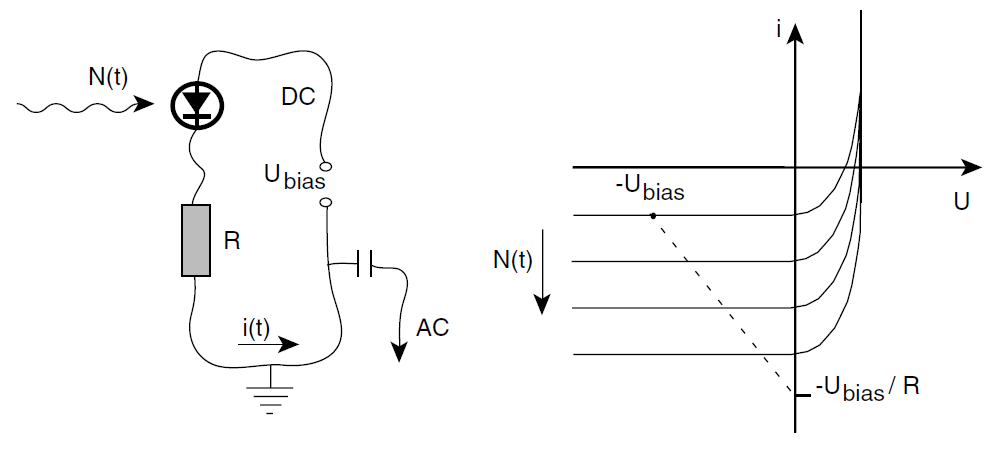
\includegraphics[width=1\linewidth]{photodector.png}
    \caption{Operação de um fotodiodo.}
    \label{photodiode}
\end{figure}

\subsubsection{Amplificadores e Ruído Eletrônico}

Os seguintes ruídos são introduzidos por um fotodiodo ao circuito:

\begin{itemize}
    \item \textbf{Dark noise}: $\Delta i(t)^2_{dark}$
    \item \textbf{Thermal noise}: $\Delta i(t)^2_{th}\approx 4k_BTB/R$.
    \item \textbf{Amplifier Noise}: $\Delta i(t)^2_{amp}\approx 2eGBF$. G é o ganho de tensão é um fator de ruído.
\end{itemize}

A intenção é obter:

\begin{equation}
    \Delta i(t)^2_{el}=\Delta i(t)^2_{dark}+\Delta i(t)^2_{th}+\Delta i(t)^2_{amp} \ll \Delta i(t)^2_{opt}
\end{equation}

O último termo contém a informação que efetivamente queremos medir.

\begin{figure}[H]
    \centering
    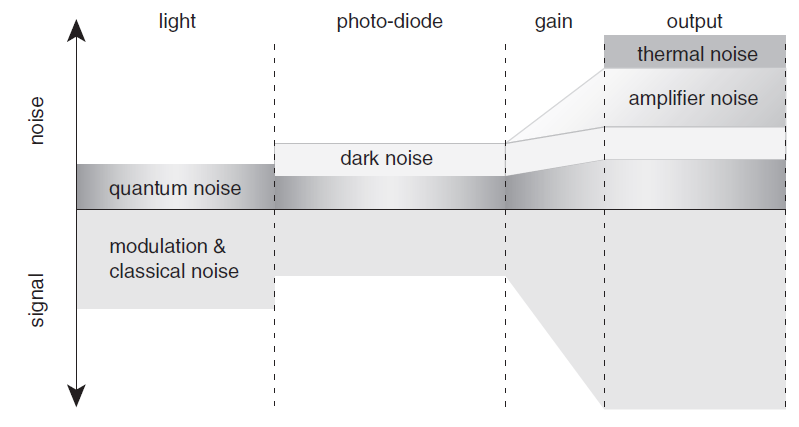
\includegraphics[width=0.7\linewidth]{noise-signal plot.png}
    \caption{As contribuições de sinal e ruído em um fotodector.}
    \label{noise.signal.plot}
\end{figure}

\subsubsection{Análise Espectral de Fotocorrentes}

\begin{itemize}
    \item O propósito do ESA (electronic spectrum analyser) é medir a mostrar a composição espectral $p_i(\Omega)$ da potência de um sinal elétrico $i(t)$.
    \item A resposta espectral do analisador é dada pela função $res(\Omega)$ que tem uma largura definida pela  \textbf{resolution bandwidth}.
    \item A potência medida é:
    \begin{equation*}
        p_i(\Omega)=\text{Média no Tempo} \Big(\int{res(\Omega)i(\Omega)R d\Omega}\Big)^2
    \end{equation*}
    \item O ESA é construído em torno da detecção heterodina (discutida em maiores detalhes à frente). O resultado da medição é uma \textbf{distribuição com média $\mu_{disp}$}, do qual deduzimos a densidade espectral $p_i(\Omega)$ da fotocorrente.
    \begin{equation}
        \mu_{disp}=\sigma^2_{noise}+C_SS^2_{sig}
    \end{equation}
    \item Definimos o \textbf{Signal to Noise Ratio} (SNR):
    \begin{equation}
        SNR=\frac{\mu_{disp}(\text{signal}+\text{noise})-\mu_{noise}(\text{noise})}{\mu_{disp}(\text{noise})}
    \end{equation}
\end{itemize}

\todo[inline]{Completar: (1) Operação do analisador eletrônico de espectro; (2) Definição do SNR}

\section{Quantum Noise: Basic Measurements and Techniques}

\subsection{Detecção e Calibração de Ruído Quântico}

A intenção dessa seção é desenvolver métodos experimentais para interpretar o espectro de ruído eletrônico, distinguir ruído quântico do ruído técnico comum e calibrar medidas de ruído. As seguintes técnicas serão discutidas:

\begin{itemize}
    \item Detecção Direta
    \item Detecção Balanceada
    \item Detecção Homodina
\end{itemize}

\subsection{Detecção Direta}

Na detecção direta, a luz é medida diretamente por um único detector, associado a um amplificador, e o resultado é avaliado em um ESA.

A detecção direta dá uma potência elétrica $p_i$ para o ruído, que idealmente seria totalmente decorrente do ruído quântico. Há entretanto, uma série de entraves para essa condição ideal: (1) ruído eletrônico; (2) Resposta AC; (3) Eficiências; (4) Saturação de Potência; (5) Saturação dos Amplificadores.

\subsection{Detecção Balanceada}



\begin{figure}[H]
    \centering
    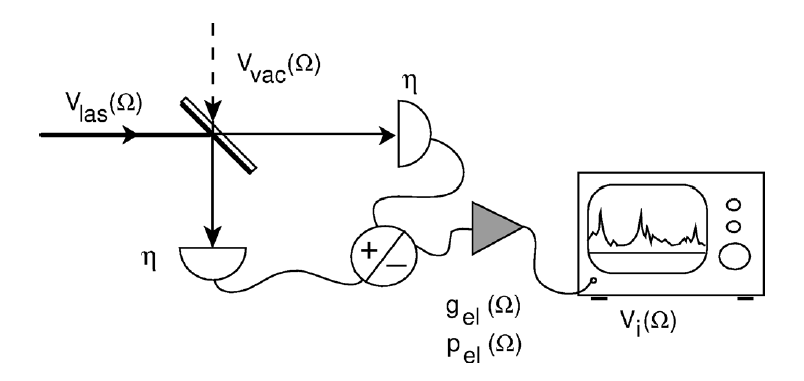
\includegraphics[width=1.0\linewidth]{balanced detection.png}
    \caption{Montagem para detecção balanceada.}
    \label{balanced.detection}
\end{figure}

\subsection{Detecção Homodina}

Na seção \ref{quatradure.amplitude}, definimos as amplitudes em quadratura de forma que a solução geral da equação de onda fica:

\begin{equation}
    \textbf{E}(\textbf{r},t)=E_0\textbf{p}(\textbf{r},t)\bigl[X_1(\textbf{r},t)\cos(\omega t)+X_2(\textbf{r},t)\sin(\omega t)\bigr]
\end{equation}

\begin{equation}
    \begin{cases}
        X_1(\textbf{r},t)=\alpha(\textbf{r},t)+\alpha^*(\textbf{r},t)\\
        X_2(\textbf{r},t)=i[\alpha(\textbf{r},t)-\alpha^*(\textbf{r},t)]\\
    \end{cases}
\end{equation}

\begin{figure}[H]
    \centering
    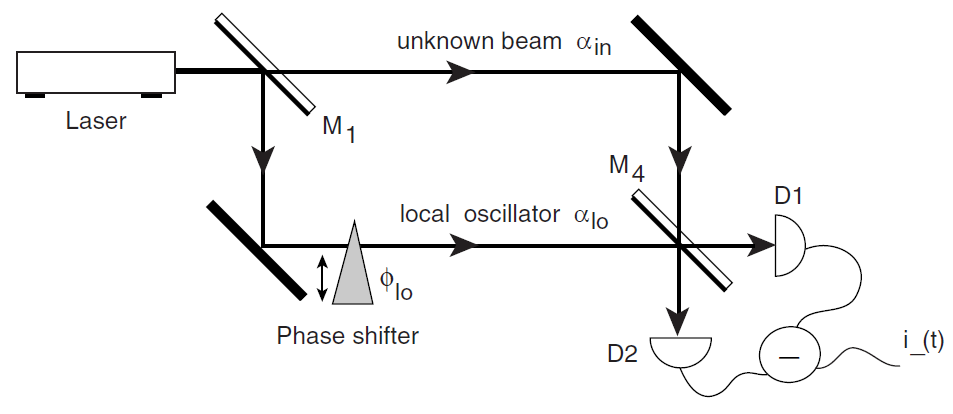
\includegraphics[width=1.0\linewidth]{homodyne detection.png}
    \caption{Montagem para detecção homodina.}
    \label{homodyne.detection}
\end{figure}

E vimos que essa notação é útil para escrever pequenas variações na amplitude e na fase de uma onda. Com efeito, podemos escrever os dois feixes da seguinte forma:

\begin{equation}
    \begin{cases}
        \alpha_{in}(t)=\alpha_{in}+\delta X_1_{in}(t)+i\delta X_2_{in}(t)\\
        \alpha_{lo}(t)=\big(\alpha_{lo}+\delta X_1_{lo}(t)+i\delta X_2_{lo}(t)\big)e^{i\phi_{lo}}
    \end{cases}
\end{equation}

Considerando que a intensidade do feixe do oscilador é muito maior que a do feixe medido $\alpha_{lo}^2\gg\alpha_{in}^2$. Nesse caso podemos supôr que toda a intensidade se deve ao oscilador, e que está igualmente distrubuída nos dois detectores:

\begin{equation}
    \abs{\alpha_{D1}}^2=\abs{\alpha_{D2}}^2=\frac{1}{2}\abs{\alpha_{lo}}^2
\end{equation}

Daí é fácil ver que:

\begin{equation}
    \begin{cases}
        \alpha_{D1}=\sqrt{1/2}\alpha_{lo}(t)+\sqrt{1/2}\alpha_{in}(t)\\
        \alpha_{D2}=\sqrt{1/2}\alpha_{lo}(t)-\sqrt{1/2}\alpha){in}(t)
    \end{cases}
\end{equation}

E a intensidade no detector 1:

\begin{equation}
    \abs{\alpha_{D1}}^2=\frac{1}{2}\Bigg[ \abs{\alpha_{lo}(t)}^2+\alpha_{lo}(t)\alpha^*_{in}(t)+\alpha_{in}(t)\alpha^*_{lo}+\abs{\alpha_{in}(t)}^2\Bigg]
\end{equation}

Fazendo algumas aproximações simples e resolvendo para a diferença entre os dois detectores:             

\begin{equation}
    i_{-}(t)\approx 2\alpha_{lo}\big(\delta X_1_{in}(t)\cos(\phi_{lo})+i\delta X_2_{in}(t)\sin(\phi_{lo})\big)
\end{equation}

\pagebreak

\section{Quantum Noise}

\pagebreak
